
\chapter{Multivariate statistics background}

Multivariate statistics will prove to be a central tool in our later analyses.  We use this chapter to gather the relevant definitions and results, concentrating mainly on the eigenvalues and eigenvectors from sample covariance matrices.  The literature in this area spans over fifty years.  We give the basic definitions and properties of the multivariate normal and Wishart distributions in Section~\ref{S:mulitivariate-definitions}.  Then, in Section~\ref{S:multivariate-classical}, we survey classical results about sample covariance matrices when the number of dimensions, $p$, is fixed and the sample size, $n$, grows to infinity.  This material is by now standard and can be found in any good multivariate statistics book.  Lastly,  in Section~\ref{S:multivariate-modern}, we survey modern asymptotics, where $n \to \infty$ and $p$ grows with $n$.  Modern multivariate asymptotics is still an active research topic, but today it is possible to give a reasonably-complete description of the objects of interest.

\section{The multivariate normal and Wishart distributions}\label{S:mulitivariate-definitions}

We start with the definition of the multivariate normal distribution and some basic properties, which can be found, for example, in \cite{muirhead1982ams}[Chapters 1--3].

\begin{definition}[Multivariate Normal Distribution]
    \label{D:multivariate-normal}
For mean vector 
\(
    \vmu \in \reals^p
\)
and positive-semidefinite covariance matrix
\(
    \mSigma \in \reals^{p\times p},
\)
a random vector 
\(
    \vX \in \reals^p
\)
is distributed from the multivariate normal distribution, denoted 
\(
    \vX 
    \sim 
    \Normal \left(
        \vmu, \,
        \mSigma
    \right)
\)
if for every fixed vector $\va \in \reals^p$, the vector
$\va^\trans \vX$ has a univariate normal distribution with mean
\(
    \va^\trans \vmu
\)
and variance
\(
    \va^\trans \mSigma \va
\).
\end{definition}

\noindent
The multivariate normal distribution is defined for any positive-semidefinite covariance matrix $\mSigma$, but it only has a density when $\mSigma$ is strictly positive definite.

\begin{proposition}
If $\vX \in \reals^p$ follows a multivariate normal distribution with mean $\vmu$ and positive-definite covariance matrix $\mSigma$, then its components have density
\begin{equation}\label{E:normal-density}
    f( \vx )
    =
    (2 \pi )^{-p/2}
    |\mSigma|^{-1/2}
    \exp\left(
        -
        \frac{1}{2}
        (\vx - \vmu)^\trans
        \mSigma^{-1}
        (\vx - \mu)
    \right).
\end{equation}
\end{proposition}

A basic fact about the multivariate normal is the following:

\begin{proposition}\label{P:scale-shift-normal}
Let 
\(
    \va \in \reals^p,
\)
\(
    \mC \in \reals^{q \times p},
\)
and say
\(
    \vX 
    \sim
    \Normal \left( 
        \vmu, \,
        \mSigma
    \right).
\)
Define $\vY = \mC \vX + \va$.  Then 
\(
    \vY
    \sim
    \Normal \left( 
        \mC \vmu + \va, \,
        \mC \mSigma \mC^\trans
    \right).
\)
\end{proposition}

\noindent
Two immediate corollaries are

\begin{corollary}\label{C:normal-orthog-invariant}
Say that
\(
    \vX 
    \sim 
    \Normal \left( 
        \vzero, \,
        \sigma^2 \mI_p
    \right)
\)
and that
\(
    \mO \in \reals^{p \times p}
\)
is an orthogonal matrix.  Then
\(
    \mO \vX \eqd \vX.
\)
\end{corollary}

\begin{corollary}
Suppose that
\(
    \vX 
    \sim 
    \Normal \left( 
        \vzero, \,
        \mSigma
    \right)
\)
and that $\mSigma = \mC \mC^\trans$ for a matrix $\mC \in \reals^{p \times p}$.
Let 
\(
    \vZ
    \sim
    \Normal \left(
        \vzero, \,
        \mI_p
    \right)
\).
Then
\(
    \mC \vZ
    \eqd
    \vX
\).
\end{corollary}    

We are often interested in estimating the underlying parameters from
multivariate normal data.  The sufficient statistics are the standard
estimates.

\begin{proposition}\label{P:normal-sufficient-stats}
Say that
\(
    \vX_1, \vX_2, \ldots, \vX_n
\) 
are independent draws from a
\(
    \Normal \left(
        \vmu, \,
        \mSigma
    \right)
\)
distribution.  Then the sample mean
\begin{equation}\label{E:sample-mean}
    \vbX_n
    \define
    \frac{1}{n}
    \sum_{i=1}^n
        \vX_i
\end{equation}
and the sample covariance
\begin{equation}\label{E:sample-covariance}
    \mS_n
    \define
    \frac{1}{n-1}
    \sum_{i=1}^n
        \left(
            \vX_i - \vbX_n
        \right)^2
\end{equation}
are sufficient statistics for $\vmu$ and $\mSigma$.
\end{proposition}

To describe the distribution of $\mS_n$, we need to introduce the 
Wishart distribution.

\begin{definition}[Wishart Distribution]\label{D:wishart}
Let $\vX_1, \vX_2, \ldots, \vX_n \in \reals^p$ be an \iid sequence of
random vectors, each distributed as
\(
    \Normal \left(
        \vzero, \,
        \mSigma
    \right).
\)
Then the matrix
\[
    \mA = \sum_{i=1}^n \vX_i \vX_i^\trans
\]
is said to have the Wishart distribution with $n$ degrees of freedom and scale parameter $\mSigma$.  We denote this by
\(
    \mA
    \sim
    \Wishart_p \left(
        n, \,
        \mSigma
    \right).
\)
\end{definition}

\noindent
When $n \geq p$ and $\mSigma$ is positive-definite, the elements of a Wishart matrix have a density.
\begin{proposition}
Suppose that
\(
    \mA
    \sim
    \Wishart_p \left(
        n, \,
        \mSigma
    \right)
\).
If $n \geq p$ and $\mSigma$ is positive-definite, then the elements of $\mA$ have a density over the space of positive-definite matrices, given by
\begin{equation}\label{E:wishart-density}
    f( \mA )
    =
    \frac{ |\mA|^\frac{n-p-1}{2} }
         { 2^\frac{np}{2} 
           |\mSigma|^\frac{n}{2} 
           \Gamma_p \left( \frac{n}{2} \right) }
    \exp \left(
        -
        \frac{1}{2}
        \tr \left(
            \mSigma^{-1} \mA
        \right)
    \right),
\end{equation}
where
\(
    \Gamma_p \left( \cdot \right)
\)
is the multivariate gamma function, computed as
\begin{equation}
    \Gamma_p \left( \frac{n}{2} \right)
    =
    \pi^{p(p-1)/4}
    \prod_{i=1}^p
        \Gamma \left(
            \frac{n + 1 - i}{2}
        \right).
\end{equation}
\end{proposition}

We can now characterize the distributions of the sufficient statistics of a sequence of \iid multivariate normal random vectors.

\begin{proposition}
Let 
\(
    \vbX_n
\) 
and 
\(
    \mS_n
\)
be defined as in Proposition~\ref{P:normal-sufficient-stats}.  Then
\(
    \vbX_n
\)
and
\(
    \mS_n
\)
are independent with
\(
    \vbX_n
    \sim
    \Normal \left(
        \mu, \,
        \frac{1}{n}
        \mSigma
    \right)
\)
and
\(
    (n-1)
    \mS_n
    \sim
    \Wishart_p \left(
        n-1, \,
        \mSigma
    \right)
\).
\end{proposition}

White Wishart matrices---those with scale parameter $\mSigma = \sigma^2 \mI_p$
are of particular interest.  We can characterize their distribution in
terms of eigenvalues and eigenvectors.

\begin{proposition}
Suppose that
\(
    \mA
    \sim
    \Wishart_p \left(
        n, \,
        \sigma^2 \mI_p
    \right)
\)
with
\(
    n \geq p
\)
and let
\(
    \mA = n \mO \mL \mO^\trans
\)
be the spectral decomposition of
\(
    \mA,
\)
with
\(
    \mL
    =
    \diag \left(
        l_1,
        l_2,
        \ldots,
        l_p
    \right)
\)
and
\(
    l_1
    >
    l_2
    >
    \cdots
    >
    l_p
    >
    0.
\)
Then $\mO$ and $\mL$ are independent, with $\mO$ Haar-distributed over
the group of $p \times p$ orthogonal matrices and the elements of $\mL$
having density
\begin{equation}\label{E:wishart-eig-density}
    \left(
        \frac{1}{2 \sigma^2 }
    \right)^{np/2}
    \frac{ \pi^{p^2/2} }
         { \Gamma_p \left( \frac{n}{2} \right) 
           \Gamma_p \left( \frac{p}{2} \right) }
    \prod_{i < j}^p
        \left| l_i - l_j \right|
    \prod_{i=1}^p
        l_i^{(n-p-1)/2}
        e^{-\tfrac{l_i}{2 \sigma^2}}
        .
\end{equation}    
\end{proposition}
\noindent
In the random matrix theory literature, with $\sigma^2 = 1$ the eigenvalue density above is sometimes referred to as the Laguerre Orthogonal Ensemble (LOE).

\section{Classical asymptotics}\label{S:multivariate-classical}

In this section we present results about sample covariance matrices when the sample size, $n$, tends to infinity, with the number of dimensions, $p$ a fixed constant.  A straightforward application of the strong law of large numbers gives us the limits of the sample mean and covariance.

\begin{proposition}\label{P:suff-stat-limits}
Let $\vX_1, \vX_2, \ldots, \vX_n$ be a sequence of \iid random vectors in $\reals^p$ with
\(
    \E \left[
        \vX_1
    \right]
    =
    \vmu
\)
and
\(
    \E \left[
        \left( \vX_1 - \vmu \right)
        \left( \vX_1 - \vmu \right)^\trans
    \right]
    =
    \mSigma.
\)
Then, as $n \to \infty$,
\[
    \vbX_n
    \define
    \frac{1}{n}
    \sum_{i=1}^n
        \vX_i
    \toas
    \vmu
\]
and
\[
    \mS_n
    \equiv
    \frac{1}{n-1}
    \sum_{i=1}^{n}
        \left( \vX_i - \vbX_n \right)
        \left( \vX_i - \vbX_n \right)^\trans
    \toas
    \mSigma.
\]
\end{proposition}

To simplify matters, for the rest of the section we will mostly work in a setting when the variables have been centered.  In this case, the sample covariance matrix takes the form
\(
    \mS_n = \frac{1}{n} \sum_{i=1}^n \vX_i \vX_i^\trans.
\)
To see that centering the variables does not change the theory in any essential way, we provide the following proposition.

\begin{proposition}
Let $\vX_1, \vX_2, \ldots, \vX_n$ be a sequence of random observations in $\reals^p$ with mean vector $\vmu$ and covariance matrix $\mSigma$.  Let
\(
    \vbX_n = \frac{1}{n} \sum_{i=1}^n \vX_i
\)
and
\(
    \mS_n
    =
    \frac{1}{n-1}
    \sum_{i=1}^n
        \left( \vX_i - \vbX_n \right) \!
        \left( \vX_i - \vbX_n \right)^\trans
\)
be the sample mean and covariance, respectively.  Define the centered
variables
\(
    \vtX_i = \vX_i - \vmu.
\)
Then
\[
    \mS_n
    =
    \frac{1}{n}
    \sum_{i=1}^n
        \vtX_i \vtX_i^\trans
    +
    \OhP\left( \frac{1}{n} \right).
\]
In particular, this implies that
\[
    \sqrt{n}
    \left(
        \mS_n - \mSigma
    \right)
    =
    \sqrt{n}
    \left(
        \frac{1}{n}
        \sum_{i=1}^n
            \vtX_i \vtX_i^\trans
        -
        \mSigma
    \right)
    + 
    \OhP \left( \frac{1}{\sqrt{n}} \right).
\]
\end{proposition}
\begin{proof}
We can write
\begin{align*}
    \mS_n &= \frac{1}{n-1}
             \sum_{i=1}^n \vtX_i \vtX_i^\trans
             +
             \frac{n}{n-1}
             \left(
                \vbX_n - \vmu
             \right)
             \left(
                \vbX_n - \vmu
             \right)^\trans \\
          &= \left(
                \frac{1}{n}
                +
                \frac{1}{n (n-1) }
             \right)
             \sum_{i=1}^n \vtX_i \vtX_i^\trans
             +
             \frac{n}{n-1}
             \left(
                \vbX_n - \vmu
             \right)
             \left(
                \vbX_n - \vmu
             \right)^\trans
\end{align*}
The result follows since
\(
    \vtX_i \vtX_i^\trans = \OhP \left( 1 \right)
\)
and
\(
    \vbX_n - \vmu 
    = 
    \OhP \left( \frac{1}{ \sqrt{n} } \right).
\)

\end{proof}

The next fact follows directly from the multivariate central limit theorem.

\begin{proposition}\label{P:sample-cov-limit}
Suppose that 
\(
    \vX_1, \vX_2, \ldots, \vX_n
\)
is a sequence of \iid random vectors in $\reals^p$ with 
\[
    \E \left[
        \vX_1 \vX_1^\trans
    \right]
    =
    \mSigma,
\]
and that for all $1 \leq i,j,i',j' \leq p$ there exists 
\(
    \Gamma_{iji'j'} < \infty
\)
with
\[
    \E \left[
        \left(
            X_{1i} X_{1j}
            -
            \Sigma_{ij}
        \right)
        \left(
            X_{1i'} X_{1j'}
            -
            \Sigma_{i'j'}
        \right)
    \right]
    =
    \Gamma_{iji'j'}.
\]
If
\(
    \mS_n
    =
    \frac{1}{n}
    \sum_{i=1}^n
        \vX_i \vX_i^\trans,
\)
then
\(
    \sqrt{n}
    \vecm \left( 
        \mS_n - \mSigma 
    \right)
    \tod
    \vecm \left( 
        \mG
    \right),
\)
where $\mG$ is a random $p \times p$ symmetric matrix with 
\(
    \vecm \left( \mG \right)
\)
a mean-zero multivariate normal having covariance
\(
    \cov \left(
        G_{ij}, \,
        G_{i'j'}
    \right)
    =
    \Gamma_{iji'j'}.
\)
\end{proposition}

\noindent
If the elements of $\vX_1$ have vanishing first and third moments (for instance if
\(
    \vX_1 \eqd - \vX_1
\)
), and if
\(
    \E \left[
        \vX_1 \vX_1^\trans
    \right]
    =
    \diag \left(
        \lambda_1,
        \lambda_2,
        \ldots,
        \lambda_p
    \right),
\)
then $\Gamma_{iji'j'}$ simplifies to
\begin{subequations}
\begin{align}
    \Gamma_{iiii} &= \E \left[ X_{1i}^4 \right] - \lambda_i^2 \quad 
                         &&\text{for $1 \leq i \leq p$}, \\
    \Gamma_{ijij} = \Gamma_{ijji} &= \E \left[ X_{1i}^2 X_{1j}^2 \right]
                         &&\text{for $ 1 \leq i,j \leq p$, $i \neq j$;}
\end{align}
\end{subequations}
all other values of $\Gamma_{iji'j'}$ are $0$.  In particular, this
implies that the elements of $\vecm \left( \mG \right)$ are independent.
If we also have that $\vX_1$ is multivariate normal, then 
\begin{subequations}
\begin{align}
    \Gamma_{iiii} &= 2 \lambda_i^2
                         &&\text{for $1 \leq i \leq p$, and} \\    
    \Gamma_{ijij} = \Gamma_{ijji} &= \lambda_i \lambda_j
                         &&\text{for $ 1 \leq i,j \leq p$, $i \neq j$.}
\end{align}
\end{subequations}


It is inconvenient to study the properties of the sample covariance matrix when the population covariance
\(
    \mSigma
\)
is not diagonal.  By factorizing
\(
    \mSigma
    =
    \mPhi
    \mLambda
    \mPhi^\trans
\)
for orthogonal $\mPhi$ and diagonal $\mLambda$, we can introduce
\(
    \vtX_i
    \define
    \mPhi^\trans \vX_i
\)
to get
\(
    \E \left[
        \vtX_i
        \vtX_i^\trans
    \right]
    =
    \mLambda
\)
and
\(
    \mS_n
    =
    \mPhi
    \left(
        \frac{1}{n}
        \sum_{i=1}^n
            \vtX_i \vtX_i^\trans
    \right)
    \mPhi^\trans.
\)
With this transformation, we can characterize the distribution of $\mS_n$ completely in terms of
\(
    \frac{1}{n}
    \sum_{i=1}^n
        \vtX_i \vtX_i^\trans.
\)


The next result we present is about the sample principal compoents.  It is motivated by Proposition~\ref{P:sample-cov-limit} and is originally due to Anderson~\cite{anderson1963atp}, though he does not state result quite like this.  

\begin{theorem}\label{T:eigen-random-perturb}
For $n\to \infty$ and $p$ fixed, let $\mS_1, \mS_2, \ldots, \mS_n$ be a sequence of random symmetric $p \times p$ matrices with 
\(
    \sqrt{n} \vecm \left( \mS_n - \mLambda \right)
    \tod
    \vecm \left( \mG \right),
\)
for a deterministic
\(
    \mLambda = \diag\left( \lambda_1, \lambda_2, \ldots, \lambda_p \right)
\)
having $\lambda_1 > \lambda_2 > \cdots > \lambda_p$ and a random symmetric matrix $\mG$.
Let
\(
    \mS_n = \mU_n \mL_n \mU_n^\trans
\)
be the eigendecomposition of $\mS_n$, with
\(
    \mL_n = \diag\left( l_{n,1}, l_{n,2}, \ldots, l_{n,p} \right)
\)
and
\(
    l_{n,1} \geq l_{n,2} \geq \cdots \geq l_{n,p}.
\)
If $\mG = \OhP\left( 1 \right)$, and the signs of $\mU_n$ are chosen so that $U_{n,ii} \geq 0$ for $1 \leq i \leq p$, then the elements of $\mU_n$ and $\mL_n$ converge jointly as
\begin{subequations}
\begin{alignat}{2}
    \sqrt{n}
    \left( U_{n, ii} - 1 \right)
        &\toP 0
                &&\quad \text{for $1 \leq i \leq p$,} \\
    \sqrt{n}
    U_{n, ij}
        &\tod -
              \frac{ G_{ij} }{ \lambda_i - \lambda_j }
                &&\quad \text{for $1 \leq i,j \leq p$ with $i \neq j$, and} \\
    \sqrt{n}
    \left( l_{n,i} - \lambda_i \right)
        &\tod G_{ii}
                &&\quad \text{for $1 \leq i \leq p$.} \qedhere
\end{alignat}
\end{subequations}
\end{theorem}
\noindent
More generally, Anderson treats the case when the $\lambda_i$ are not all unique.  The key ingredient to Anderson's proof is a perturbation lemma, which we will state and prove.

\begin{lemma}\label{L:eigen-perturb}
For 
\(
    n \to \infty
\)
and fixed
\(
    p
\)
let
\(
    \mS_1, \mS_2, \ldots, \mS_n \in \reals^{p\times p}
\) 
be a sequence of symmetric matrices of the form
\[
    \mS_n 
    = 
    \mLambda
    +
    \frac{1}{\sqrt{n}}
    \mH_n
    +
    \oh\left( \frac{1}{\sqrt{n}} \right),
\]
where
\(
    \mLambda
    =
    \diag \left(
        \lambda_1,
        \lambda_2,
        \ldots,
        \lambda_p
    \right)
\)
with 
\(
    \lambda_1 > \lambda_2 > \cdots > \lambda_p
\) 
and
\(
    \mH_n = \Oh\left( 1 \right).
\)
Let $\mS_n = \mU_n \mL_n \mU_n^\trans$ be the eigendecomposition of $\mS_n$, with
\(
    \mL_n
    =
    \diag \left(
        l_{n,1}, l_{n,2}, \ldots, l_{n,p}
    \right).
\)
Further suppose that $U_{n,ii} \geq 0$ for $1 \leq i \leq p$ and
\(
    l_{n,1} > l_{n,2} > \cdots > l_{n,p}.
\)
Then for all $1 \leq i,j \leq p$ and $i \neq j$ we have
\begin{subequations}
\begin{align}
    U_{n,ii} 
        &= 1 
           + 
           \oh \left( 
               \frac{ 1 }{ \sqrt{n} }
           \right), \\
    U_{n,ij}
        &= -
           \frac{ 1 }{ \sqrt{n} }
           \frac{ H_{n,ij} }{ \lambda_i - \lambda_j }
           +
           \oh \left(
               \frac{ 1 }{ \sqrt{n} }
           \right), \quad \text{and} \\
    l_{n,i}
        &= \lambda_i
           + 
           \frac{ H_{n,ii} }{ \sqrt{n} }
           +
           \oh \left(
               \frac{ 1 }{ \sqrt{n} }
           \right).
\end{align}
\end{subequations}
\end{lemma}
\begin{proof}
Define $p\times p$ matrices $\mE_n$, $\mF_n$, and $\mDelta_n$ so that
\begin{align}
    \mE_n
        &=
        \diag \left(
            U_{n,11},
            U_{n,22},
            \ldots,
            U_{n,pp}
        \right), \\
    \mF_n 
        &= 
        \sqrt{n} \left( \mU_n - \mE_n \right), \\
    \mDelta_{n}
        &=
        \sqrt{n} \left( \mL_n - \mLambda \right), \\
\intertext{giving}
    \mU_n
        &= \mE_n + \frac{1}{\sqrt{n}} \mF_n, \quad \text{and} \notag \\
    \mL_n
        &= \mLambda + \frac{1}{\sqrt{n}} \mDelta_{n}. \notag
\end{align}
We have that 
\begin{align}
    \mS_n 
    &= \mLambda 
       + \frac{1}{\sqrt{n}} \mH_n 
       + \oh \left( \frac{1}{\sqrt{n}}\right) \notag \\
    &= \mU_n \mL_n \mU_n^\trans \notag \\
    &= \mE_n \mLambda \mE_n^\trans
       + 
       \frac{1}{\sqrt{n}} \left(
           \mE_n \mDelta_n \mE_n^\trans
           +
           \mF_n \mLambda \mE_n^\trans
           +
           \mE_n \mLambda \mF_n^\trans
       \right)
       +
       \frac{1}{n}
       \mM_n \label{L:eigen-perturb:E:eigen-perturb}
\end{align}
where the elements of $\mM_n$ are sums of $\Oh\left( p \right)$ terms, with each term a product of elements taken from $\mE_n$, $\mF_n$, $\mLambda$, and $\mDelta_n$.  Also,
\begin{align}
    \mI_p
    &= \mU_n \mU_n^\trans \notag \\
    &= \mE_n \mE_n^\trans
       + 
       \frac{1}{\sqrt{n}} \left(
           \mF_n \mE_n^\trans
           +
           \mE_n \mF_n^\trans
       \right)
       + 
       \frac{1}{n}
       \mW_n, \label{L:eigen-perturb:E:orthog-perturb}
\end{align}
where $\mW_n = \mF_n \mF_n^\trans$.
From \eqref{L:eigen-perturb:E:orthog-perturb} we see that for $1 \leq i,j \leq p$ and $i \neq j$ we must have
\begin{subequations}
\begin{align}
    1 &= E_{n,ii}^2 
         + 
         \frac{1}{n} W_{n,ii}, 
         \quad \text{and}
         \label{L:eigen-perturb:E:orthog-perturb-1} \\
    0 &= E_{n,ii} F_{n,ji} 
         + 
         F_{n,ij} E_{n,jj} 
         + 
         \frac{1}{\sqrt{n}} W_{n,ij}.
         \label{L:eigen-perturb:E:orthog-perturb-2}
\end{align}
\end{subequations}
Substituting
\(
    E_{n,ii}^2 = 1 - \frac{1}{n} W_{n,ii}
\)
into equation~\eqref{L:eigen-perturb:E:eigen-perturb}, we get
\begin{subequations}
\begin{align}
    H_{n,ii} 
        &= E_{n,ii} \Delta_{n,ii} E_{n,ii}
           + 
           \frac{1}{\sqrt{n}} \left(
                M_{n,ii} - \lambda_i W_{n,ii}
           \right)
           +
           \oh \left( 1 \right), \quad \text{and} 
           \label{L:eigen-perturb:E:eigen-perturb-1} \\
    H_{n,ij}
        &= \lambda_j E_{n,jj} F_{n,ij}
           +
           \lambda_i F_{n,ji} E_{n,ii} 
           +
           \frac{1}{\sqrt{n}} M_{n,ij}
           +
           \oh \left( 1 \right).
           \label{L:eigen-perturb:E:eigen-perturb-2} 
\end{align}
\end{subequations}
Equations~\eqref{L:eigen-perturb:E:orthog-perturb-1}--\eqref{L:eigen-perturb:E:eigen-perturb-2} admit the solution
\begin{subequations}
\begin{align}
    E_{n,ii} 
        &= 1 + \oh\left(\frac{1}{\sqrt{n}}\right), \\
    F_{n,ij}
        &= -
           \frac{ H_{n,ij} }
                { \lambda_i - \lambda_j }
           +
           \oh \left( 1 \right), \quad \text{and} \\
    \Delta_{n,ii}
        &= H_{n,ii} + \oh\left( 1 \right).
\end{align}
\end{subequations}
\end{proof}

An application of the results of this section is the following theorem, which describes the behavior of principal components analysis for large $n$ and fixed $p$.

\begin{theorem}
Let $\vX_1, \vX_2, \ldots, \vX_n$ be a sequence of \iid 
\(
    \Normal \left(
        \vmu, \,
        \mSigma
    \right)
\)
random vectors in $\reals^p$, with sample mean
\(
    \vbX_n
\)
and sample covariance
\(
    \mS_n.
\)
Let $\mSigma = \mPhi \mLambda \mPhi^\trans$ be the eigendecomposition
of $\mSigma$, with
\(
    \mLambda = \diag \left(
        \lambda_1,
        \lambda_2,
        \ldots,
        \lambda_p
    \right)
\)
and
\(
    \lambda_1 > \lambda_2 > \cdots > \lambda_p > 0
\).
Similarly, let $\mS_n = \mU_n \mL_n \mU_n^\trans$ be the eigendecomposition of $\mS_n$, likewise with
\(
    \mL_n = \diag \left(
        l_{n,1},
        l_{n,2},
        \ldots,
        l_{n,p}
    \right)
\),
\(
    l_1 > l_2 > \cdots > l_p
\),
and signs chosen so that
\(
    \left( \mPhi^\trans \mU_n \right)_{ii} \geq 0
\)
for $1 \leq i \leq p$.  Then
\begin{enumerate}[(i)]
    \item $\mU_n \toas \Phi$ and $l_{n,i} \toas \lambda_i$ for
        $1 \leq i \leq p$.
    \item Jointly for all $1 \leq i \leq p$,
        \[
            \sqrt{n} \left( l_{n,i} - \lambda_i \right) 
            \tod 
            \Normal\left( 0, \, 2 \lambda_i^2 \right)
        \]
        and
        \[
            \sqrt{n} \left( \mPhi^\trans \mU_n - \mI_p \right) \tod \mF,
        \]
        where $\mF$ is a skew-symmetric matrix independent of the
        eigenvalue limits with elements above the diagonal independent of
        each other and distributed as 
        \[
            F_{ij}
            \sim
            \Normal \left(
                0, \,
                \frac{\lambda_i \lambda_j}
                     {\left( \lambda_i - \lambda_j \right)^2}
            \right),
            \quad
            \text{for all $1 \leq i < j \leq p$.}
        \]
\end{enumerate}
\end{theorem}
\begin{proof}
Part (i) is a restatement of Proposition~\ref{P:suff-stat-limits}.  Part (ii) follows from Proposition~\ref{P:sample-cov-limit} and Theorem~\ref{L:eigen-perturb}.
\end{proof}


\section{Modern asymptotics}\label{S:multivariate-modern}

We now present some results about sample covariance matrices when both the sample size, $n$, and the dimensionality, $p$, go to infinity.  Specifically, most of these results suppose that $n \to \infty$, $p \to \infty$, and 
\(
    \frac{n}{p} \to \gamma
\)
for a fixed constant
\(
    \gamma \in \left( 0, \infty \right).
\)
There is no widely-accepted name for $\gamma$, but we will adopt the terminology of Mar\v{c}enko and Pastur \cite{marcenko1967des} and call it the \emph{concentration}.

Most of the random matrix theory literature concerning sample covariance matrices is focused on eigenvalues.  Given a sequence of sample covariance matrices $\mS_1, \mS_2, \ldots, \mS_n$, with $\mS_n \in \reals^{p\times p}$ and $p = p(n)$ these results generally come in one of two forms.  If we label the eigenvalues of $\mS_n$ as
\(
    l_{n,1}, l_{n,2}, \ldots, l_{n,p},
\)
with $l_{n,1} \geq l_{n,2} \geq \cdots \geq l_{n,p}$, then we can define
a random measure
\[
    F^{S_n} = \frac{1}{p} \sum_{i=1}^p \delta_{l_{n,i}}.
\]
This measure represents a random draw from the set of eigenvalues of $\mS_n$ that puts equal weight on each eigenvalue.  It is called the \emph{spectral measure} of $\mS_n$.  Results about $F^{S_n}$ are generally called results about the ``bulk'' of the spectrum.  

The second major class of results is concerned with the behavior of the
extreme eigenvalues $l_{n,1}$ and $l_{n,p}$. Results of this type are called
``edge'' results.

\subsection{The bulk of the spectrum}

To work in a setting where the dimensionality $p$, grows with the sample size, $n$, we introduce a triangular array of sample vectors.  The sample covariance matrix $\mS_n$ is of dimension $p\times p$ and is formed from row $n$ of a triangular array of independent random vectors,  
$\vX_{n,1}, \vX_{n,2}, \ldots, \vX_{n,n}$.  Specifically,
\(
    \mS_n
    =
    \frac{1}{n}
    \sum_{i=1}^n \vX_{n,i} \vX_{n,i}^\trans.
\)
We let $\mX_n$ be the $n \times p$ matrix
\(
    \mX_n
    =
    \left(
    \begin{matrix}
        \vX_{n,1}^\trans \\
        \vX_{n,2}^\trans \\
        \vdots \\
        \vX_{n,n}^\trans
    \end{matrix}
    \right),
\)
so that 
\(
    \mS_n
    =
    \frac{1}{n}
    \mX_n^\trans \mX_n.
\)
Most asymptotic results about sample covariance matrices are expressed in terms of $\mX_n$ rather than $\mS_n$.  For example, the next theorem about the spectral measure of a large covariance matrix is stated this way.

\begin{theorem}\label{T:mp-limit}
Let $\mX_1, \mX_2, \ldots, \mX_n$ be a sequence of random matrices of increasing dimension as $n \to \infty$, so that $\mX_n \in \reals^{n\times p}$ and $p = p(n)$.
Define $\mS_n = \frac{1}{n} \mX_n^\trans \mX_n$.  If the elements of $\mX_n$ are \iid with $\E| X_{n,11} - \E X_{n,11} |^2 = 1$ and $\frac{n}{p} \to \gamma > 0$, then the empirical spectral measure $F^{\mS_n}$ almost surely converges in distribution to a deterministic probability measure.  This measure, denoted
$\FMP_\gamma$, is called the Mar\v{c}enko-Pastur Law.  For $\gamma \geq 1$ it
has density
\begin{equation}
    \fMP_\gamma(x)
    =
    \frac{\gamma}{2 \pi x}
    \sqrt{(x - a)(b - x)},
    \quad
    a \leq x \leq b,
\end{equation}
where
\(
    a = \left( 1 - \frac{1}{\sqrt{\gamma}} \right)^2
\)
and
\(
    b = \left( 1 + \frac{1}{\sqrt{\gamma}} \right)^2.
\)
When $\gamma < 1$, there is an additional point-mass of $(1 - \gamma)$ at the origin.
\end{theorem}

\noindent
Figure~\ref{F:mp-law} shows the density $\fMP_\gamma(x)$ for different values
of $\gamma$.  The reason for choosing the name ``concentration'' to refer to $\gamma$ becomes apparent in that for larger values of $\gamma$, $\FMP_\gamma$ becomes more and more concentrated around its mean.

The limiting behavior of the empirical spectral measure of a sample covariance matrix was originally studied by Mar\v{c}enko and Pastur~\cite{marcenko1967des} in 1967.  Since then, several papers have refined these results, including Grenander and Silverstein~\cite{grenander1977san}, Wachter~\cite{wachter1978slr},
 Jonsson~\cite{jonsson1982slt}, Yin and Krishnaiah~\cite{yin1983lte},
Yin~\cite{yin1986lsd}, Silverstein and Bai~\cite{silverstein1995ede}, and
Silverstein~\cite{silverstein1995sce}.  These papers either proceed via a combinatorial argument involving the moments of the matrix elements, or else they employ a tool called the Stieltjes transform.  Theorem~\ref{T:mp-limit} is a simplified version of Silverstein and Bai's main result, which more generally considers complex-valued random variables and allows the columns of $\mX_n$ to have heterogeneous variances.

\begin{figure}
    \centering
    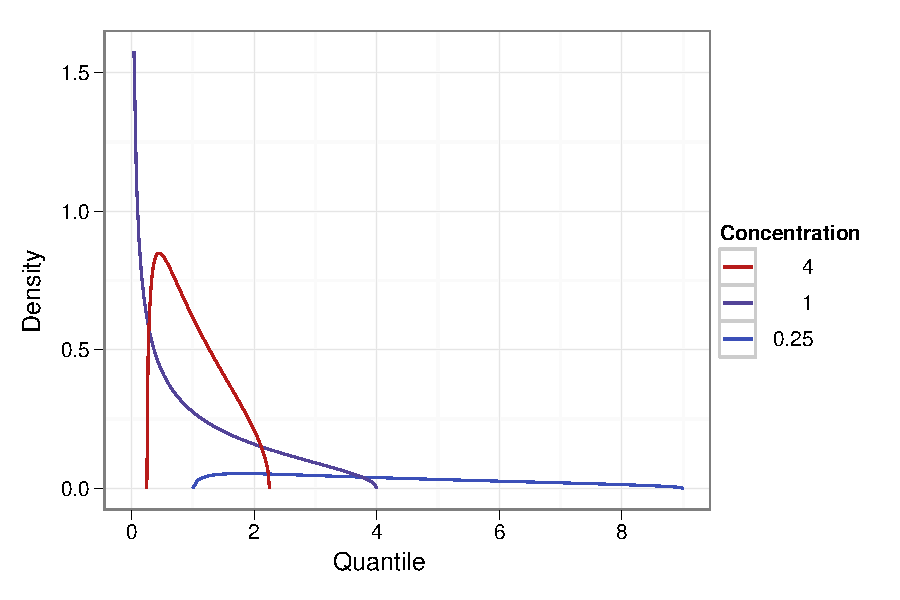
\includegraphics{mp-law}
    \caption{
        \captiontitle{The Mar\v{c}enko-Pastur Law}
        Density, $\fMP_\gamma(x)$, plotted against quantile, $x$,
        for concentration $\gamma = 0.25$, $1$, and $4$.  Concentration
        is equal to the number of samples per dimension. For $\gamma < 1$,
        there is an addition point-mass of size $(1 - \gamma)$ at $x = 0$.
    }\label{F:mp-law}
\end{figure}

The meaning of the phrase ``$F^{\mS_n}$ converges almost-surely in distribution to $\FMP_\gamma$'' is that for all $x$ which are continuity points of $\FMP_\gamma$,
\begin{equation}\label{E:spectral-measure-limit-point}
    F^{\mS_n} \left(
        x
    \right)
    \toas
    \FMP_\gamma \left(
        x
    \right).
\end{equation}
Equivalently, Theorem~\ref{T:mp-limit} can be stated as a strong law of large numbers.

\begin{corollary}[Wishart LLN]\label{C:wishart-lln}
    Let $\mX_n$ and $\{ l_{n,i} \}_{i=1}^{p}$ be as in 
    Theorem~\ref{T:mp-limit}.  Let $g : \reals \to \reals$ be any
    continuous bounded function.  Then
    \begin{equation}\label{E:wishart-functional-limit}
        \frac{1}{p}
        \sum_{i=1}^p
            g \left( l_{n,i} \right)
        \toas
        \int
            g(x)
            \,
            d\FMP_\gamma ( x ).
    \end{equation}
\end{corollary}

Concerning convergence rates for the quantities in Theorem~\ref{T:mp-limit},  Bai et al. \cite{bai2003crs} study the total variation distance between $F^{\mS_n}$ and $\FMP_\gamma$.  Under suitable conditions on $X_{11}$ and $\gamma$, they show that
\(
    \| F^{\mS_n} - \FMP_\gamma \|_\text{TV}
    =
    \OhP\left( n^{-2/5} \right)
\)
and
\(
    \| F^{\mS_n} - \FMP_\gamma \|_\text{TV}
    =
    \Ohas\left( n^{-2/5 + \varepsilon} \right)
\)
for any $\varepsilon > 0$.
Guionnet and Zeitouni \cite{guionnet2000csm} give concentration of measure results.  If $X_{11}$ satisfies a Poincar\'e inequality and $g$ is Lipschitz, they show that for $\delta$ large enough,
\begin{equation}\label{E:wishart-ldp}
    -
    \frac{1}{n^2}
    \log \Prob\left\{ 
        \left|
            \int g(x) \, dF^{\mS_n}(x) - \int g(x) \, d\FMP_\gamma(x)
        \right|
        >
        \delta
    \right\}
    =
    \Oh\left(
        \delta^2
    \right),
\end{equation}
with an explicit bound on the error. If one is willing to assume that the elements of $\mX_n$ are Gaussian, then Hiai and Petz~\cite{hiai1998edw} give an exact value for the quantity in \eqref{E:wishart-ldp}.  Guionnet~\cite{guionnetlds} gives a survey of other large deviations results.  

It is interesting to look at the scaled behavior in equation~\eqref{E:wishart-functional-limit} when the quantities are scaled by $p$.  Indeed one can prove a Central Limit Theorem (CLT) for functionals of eigenvalues.

\begin{theorem}[Wishart CLT]\label{T:wishart-clt}
    Let $\mX_1, \mX_2, \ldots, \mX_n$ be a sequence of random $n\times p$ 
    matrices with $p = p(n)$.  Assume that $\mX_n$ has \iid elements and that 
    $\E\left[ X_{n,11} \right] = 0$ and $\E\left[ X_{n,11}^2 \right] = 1$.  
    Define $\mS_n = \frac{1}{n} \mX_n^\trans \mX_n$ and let $F^{\mS_n}$ be its 
    spectral measure.  If $n \to \infty$, $\frac{n}{p} \to \gamma$ and $g_1, 
    g_2, \ldots, g_k$ 
    are real-valued functions analytic on the support of $\FMP_\gamma$, then 
    the sequence of random vectors
    \begin{multline*}
        p
        \cdot
        \Big(
	    \int g_1(x) \, dF^{\mS_n}(x)
	    -
            \int g_1(x) \, d\FMP(x), \\
	    \int g_2(x) \, dF^{\mS_n}(x)
	    -
	    \int g_2(x) \, d\FMP(x),
	    \ldots, \\
            \int g_k(x) \, dF^{\mS_n}(x)
	    -
            \int g_k(x) \, d\FMP(x),
	\Big)
    \end{multline*}
    is tight.
    Moreover, if $\E \left[ X_{n,11}^4 \right] = 3$, then the sequence 
    converges in distribution to a multivariate normal with mean $\vmu$ and 
    covariance $\mSigma$, where 
    \begin{equation}\label{E:wishart-clt-mean}
        \mu_i
	    =
	    \frac{ g_i(a) + g_i(b) }
                 { 4 }
	    -
            \frac{1}{2 \pi}
	    \int_{a}^{b}
	        \frac{ g_i(x) }
	             { \sqrt{(x-a)(b-x)} }
                \,
                dx
    \end{equation}
    and
    \begin{equation}\label{E:wishart-clt-cov}
    	\Sigma_{ij}
    	=
    	-
    	\frac{1}{2 \pi^2}
    	\iint
    	    \frac{g_i(z_1) g_j(z_2)}
    	         {\left( m(z_1) - m(z_2) \right)^2}
    	    \frac{d}{dz_1} m(z_1)
    	    \frac{d}{dz_2} m(z_2)
    	    dz_1 dz_2.
    \end{equation}
    In equations~\eqref{E:wishart-clt-mean}~and~\eqref{E:wishart-clt-cov},
    $a = (1 - \gamma^{-1/2})^2$ and $b = (1 + \gamma^{-1/2})^2$.  The 
    integrals in~\eqref{E:wishart-clt-cov} are contour integrals enclosing the 
    support of $\FMP_\gamma$, and
    \begin{equation}
        m(z)
        =
	    \frac{-(z + 1 - \gamma^{-1}) + \sqrt{(z-a)(z-b)}}{2 z},
    \end{equation}
    with the square root defined to have positive imaginary part when
    $\Im z > 0$.
\end{theorem}

\noindent
The case when $\E\left[ X_{n,11}^4 \right] = 3$ is of particular interest
because it arises when $X_{n,11} \sim \Normal\left( 0, 1 \right)$.
This theorem was proved by Bai and Silverstein~\cite{bai2004clt}, and can
be considered a generalization of the work by Johnsson~\cite{jonsson1982slt}.
In computing the variance integral~\eqref{E:wishart-clt-cov}, it is useful to know that $m$ satisfies
the identities 
\[
    m(\bar z) = \overline{m (z) },
\]
and
\[
    z = - \frac{1}{m(z)} + \frac{\gamma^{-1}}{m(z) + 1}.
\]
Bai and Silverstein show how to computing the limiting means and variances
for $g(x) = \log x$ and $g(x) = x^r$.  They also derive a similar CLT when
the elements of $\mX_n$ are correlated.


\subsection{The edges of the spectrum}

We now turn our attention to the extreme eigenvalues of a sample covariance
matrix.  It seems plausible that if $F^{\mS_n} \tod \FMP_\gamma$, then the
extreme eigenvalues of $\mS_n$ should converge to the edges of the support
of $\FMP_\gamma$.  Indeed, under suitable assumptions, this is exactly what
happens.  For the largest eigenvalue, work on this problem started with Geman~\cite{geman1980ltn}, and his assumptions were further weekend by Jonsson~\cite{jonsson1983ole} and Silverstein~\cite{silverstein1984ole}.
Yin et al.~\cite{yin1988lle} prove the result under the weakest possible
conditions \cite{bai1988nle}.

\begin{theorem}\label{T:max-wishart-eig-limit}
    Let $\mX_1, \mX_2, \ldots, \mX_n$ be a sequence of random matrices of
    increasing dimension, with $\mX_n$ of size $n \times p$, $p = p(n)$, 
    $n \to \infty$, and
    $\frac{n}{p} \to \gamma \in (0,\infty)$.  Let $\mS_n = \frac{1}{n} \mX_n^\trans \mX_n$ and 
    denote its eigenvalues by 
    $l_{n,1} \geq l_{n,2} \geq \cdots \geq l_{n,p}$.  If the 
    elements of $\mX_n$ are 
    \iid with $\E X_{n,11} = 0$, $\E X_{n,11}^2 = 1$, and
    $\E X_{n,11}^4 < \infty$, then
    \[
        l_{n,1} \toas \left( 1 + \gamma^{-1/2} \right)^2.
    \]
\end{theorem}

For the smallest eigenvalue, the first work was by Silverstein~\cite{silverstein1985sel}, who gives a result when 
$X_{n,11} \sim \Normal\left( 0,\, 1 \right)$.  Bai and Yin~\cite{bai1993lse} proved a theorem that mirrors Theorem~\ref{T:max-wishart-eig-limit}.

\begin{theorem}\label{T:min-wishart-eig-limit}
    Let $\mX_n$, $n$, $p$, and $\{ l_{n,i} \}_{i=1}^p$ be as in
    Theorem~\ref{T:max-wishart-eig-limit}.  If $\E X_{n,11}^4 < \infty$ and
    $\gamma \geq 1$, then
    \[
        l_{n,p} \toas \left( 1 - \gamma^{-1/2} \right)^2.
    \]
    With the same moment assumption on $X_{n,11}$, if $0 < \gamma < 1$, then
    \[
        l_{n,p-n+1} \toas \left( 1 - \gamma^{-1/2} \right)^2.
    \]
\end{theorem}

\noindent
For the case when the elements of $\mX_n$ are correlated, Bai and Silverstein~\cite{bai1998neo} give a general result that subsumes Theorems~\ref{T:max-wishart-eig-limit}~and~\ref{T:min-wishart-eig-limit}.

After appropriate centering and scaling, the largest eigenvalue of a white
Wishart matrix converges weakly to a random variable with known distribution.
Johansson~\cite{johansson2000sfa} proved this statement and identified the
limiting distribution for complex white Wishart matrices.  Johnstone~\cite{johnstone2001dle} later provided an analogous result for real matrices.  

\begin{theorem}\label{T:tw-limit-largest}
    Let $\mX_1, \mX_2, \ldots, \mX_n$ be a sequence of random matrices of
    increasing dimension, with $\mX_n \in \reals^{n\times p}$, $p = p(n)$,
    and $n \to \infty$ with $\frac{n}{p} \to \gamma \in (0, \infty)$.  Define
    $\mS_n = \frac{1}{n} \mX_n^\trans \mX_n$ and label its eigenvalues
    \(
        l_{n,1} \geq l_{n,2} \geq \cdots \geq l_{n,p}.
    \)
    If the elements of $\mX_n$ are \iid with
    \(
        X_{n,11} \sim \Normal\left( 0, \, 1 \right),
    \)
    then
    \[
        \frac{l_{n,1} - \mu_{n,p}}{\sigma_{n,p}}
        \tod
        W_1
        \sim
        \FTW_1,
    \]
    where
    \begin{align*}
        \mu_{n,p} 
            &=
            \frac{1}{n}
            \left(
                \sqrt{n - 1/2}
                +
                \sqrt{p - 1/2}
            \right), \\
        \sigma_{n,p}
            &= 
            \frac{1}{n}
            \left(
                \sqrt{n - 1/2}
                +
                \sqrt{p - 1/2}
            \right)
            \left(
                \frac{1}{\sqrt{n - 1/2}}
                +
                \frac{1}{\sqrt{p - 1/2}}
            \right)^{1/3},
    \end{align*}
    and $\FTW_1$ is the Tracy-Widom law of order 1.
\end{theorem}

\noindent
El Karoui~\cite{elkaroui2003lew} extended this result to apply when $\gamma = 0$ or $\gamma = \infty$.  With appropriate modifications to $\mu_{n,p}$ and $\sigma_{n,p}$, he later gave a convergence rate of order $(n \wedge p)^{2/3}$  for complex-valued data \cite{elkaroui2006mpt}.  Ma~\cite{ma2008atw} gave the analogous result for real-valued data.  For correlated complex normals, El Karoui~\cite{elkaroui2007twl} derived a more general version of Theorem~\ref{T:tw-limit-largest}.  

The Tracy-Widom distribution, which appears in Theorem~\ref{T:tw-limit-largest}, was  established to be the limiting distribution (after appropriate scaling) of the maximum eigenvalue from an $n \times n$ symmetric matrix with independent entries distributed as $\Normal\left( 0, \, 2 \right)$ along the main diagonal and $\Normal\left( 0, \, 1 \right)$ otherwise \cite{tracy1994lsd} \cite{tracy1996oas}.  To describte $\FTW_1$, let $q(x)$ solve the Painlev\'e II equation
\[
    q''(x) = x q(x) + 2 q^3(x),
\]
with boundary condition $q(x) \sim \Ai(x)$ as $x \to \infty$ and $\Ai(x)$ the Airy function.  Then it follows that
\[
    \FTW_1(x)
    =
    \exp \left\{
        -
        \frac{1}{2}
        \int_s^\infty
            q(x)
            +
            (x-s) q^2 (x)
            \,
            dx
    \right\}.
\]
Hastings and McLeod~\cite{hastings1980bvp} study the tail behavior of $q(x)$.  Using their analysis, one can show \cite{perry2009mre} that for $s \to -\infty$, 
\[
    \FTW_1(s)
    \sim
    \exp \left(
        -\frac{|s|^3}{24}
    \right),
\]
while for $s \to \infty$,
\[
    1 - \FTW_1(s)
    \sim
    \frac{ s^{-3/4} }
         { 4 \sqrt{ \pi } }
    \exp \left(
        -
        \frac{2}{3}
        s^{3/2}
    \right).
\]
The density of $\FTW_1$ is shown in Figure~\ref{F:tw-density}.

\begin{figure}
    \centering
    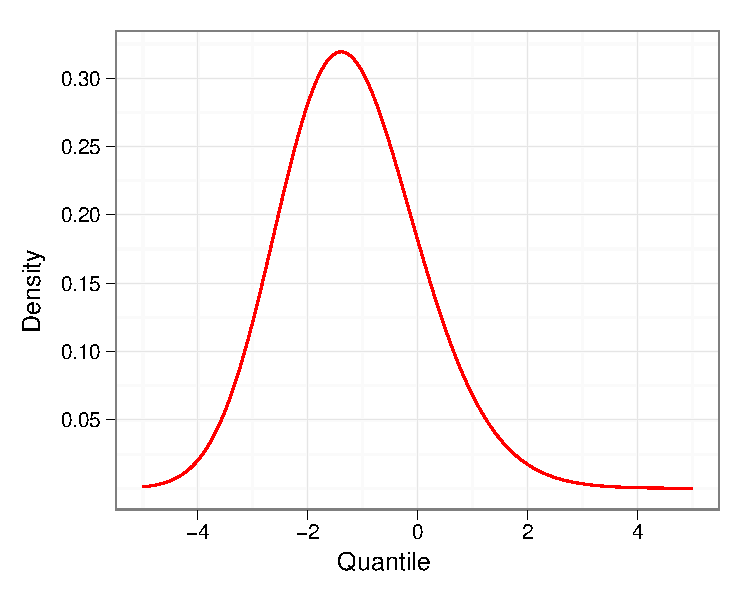
\includegraphics{tw-law}
    \caption{
        \captiontitle{The Tracy-Widom Law}
        Limiting density of the largest eigenvalue from a white Wishart
        matrix after appropriate centering and scaling.
    }
    \label{F:tw-density}
\end{figure}

A result like Theorem~\ref{T:tw-limit-largest} holds true for the smallest eigenvalue.  We define the \emph{Reflected Tracy-Widom Law} to have distribution function $\GTW_1(s) = 1 - \FTW_1(-s)$.  Then we have 

\begin{theorem}\label{T:tw-limit-smallest}
    With the same assumptions as in Theorem~\ref{T:tw-limit-largest}, if
    $\gamma \in (1,\infty)$ then
    \[
        \frac{l_{n,p} - \mu_{n,p}^-}{\sigma_{n,p}^-}
        \tod
        W_1
        \sim
        \GTW_1,
    \]
    where
    \begin{align*}
        \mu_{n,p}^-
            &=
            \frac{1}{n}
            \left(
                \sqrt{n - 1/2}
                -
                \sqrt{p - 1/2}
            \right), \\
        \sigma_{n,p}^-
            &= 
            \frac{1}{n}
            \left(
                \sqrt{n - 1/2}
                -
                \sqrt{p - 1/2}
            \right)
            \left(
                \frac{1}{\sqrt{p - 1/2}}
                -
                \frac{1}{\sqrt{n - 1/2}}
            \right)^{1/3}.
    \end{align*}
    If $\gamma \in (0, 1)$, then
    \[
        \frac{l_{n,p-n+1} - \mu_{n,p}^-}{\sigma_{n,p}^-}
        \tod
        W_1
        \sim
        \GTW_1.
    \]
\end{theorem}

\noindent
We get the result for $\gamma \in (0,1)$ by reversing the role of $n$ and $p$.
Baker et al~\cite{baker1998rme} proved the result for complex data.
Paul~\cite{paul2006dse} extended the result to real data when $\gamma \to \infty$.  Ma~\cite{ma2008atw} gives convergence rates.  In practice,
$\log l_{n,p}$ converges in distribution faster than $l_{n,p}$.  Ma recommends appropriate centering and scaling constants for $\log l_{n,p}$ to converge in distribution to a $\GTW$ random variable at rate $(n \wedge p)^{2/3}$.

Theorem~\ref{T:tw-limit-smallest} does not apply when $\frac{n}{p} \to 1$.  Edelman~\cite{edelman1988ecn} derived the limiting distribution of the smallest eigenvalue when $n = p$.  It is not known if his result holds more generally when $\frac{n}{p} \to 1$.

\begin{theorem}\label{T:edelman-limit-smallest}
    Let $\mX_n$ and $\{ l_{n,i} \}_{i=1}^p$ be as in 
    Theorem~\ref{T:tw-limit-largest}.  If $p(n) = n$, then for $t \geq 0$,
    \[
        \Prob\left\{
            n l_{n,p} \leq t
        \right\}
        \to
        \int_0^t
            \frac{1 + \sqrt{x}}{\sqrt{x}}
            e^{-(x/2 + \sqrt{x})}
            \,
            dx.
    \]
\end{theorem}

In addition to the extreme eigenvalues, it is possible to study the joint distribution of top or bottom $k$ sample eigenvalues for fixed $k$ as
$n \to \infty$.  In light of Theorem~\ref{T:mp-limit}, for fixed $k$ we must have that the top (respectively, bottom) sample eigenvalues converge almost-surely to the same limit.  Furthermore, Soshnikov~\cite{soshnikov2002nud} showed that applying the centering and scaling from Theorem~\ref{T:tw-limit-largest} to the top $k$ sample eigenvalues gives a specific limiting distribution.

It is natural to ask if the limiting eigenvalue distributions are specific to Wishart matrices, or if they apply to non-Gaussian data as well.  There is compelling evidence that the Tracy-Widom law is universal.   Soshnikov~\cite{soshnikov2002nud} extended Theorem~\ref{T:tw-limit-largest} to more general $\mX_n$ under the assumption that $X_{n,11}$ is sub-Gaussian and $n-p = \Oh(p^{1/3})$.  Tao and Vu~\cite{tao2009rmd} showed that Theorem~\ref{T:tw-limit-smallest} applies for general $X_{n,11}$ with $\E X_{n,11} = 0$ and $\E X_{n,11}^2 = 1$.


\subsection{Eigenvectors}

Relatively little attention has been focused on the eigenvectors of sample covariance matrices.  While many results are known, as of yet there is no complete characterization of the eigenvectors from a general sample covariance matrix.  Most of the difficulty in tackling the problem is that it is difficult to describe convergence properties of $\mU_n$, the $p\times p$ matrix of eigenvectors, when $n$ and $p$ go to infinity.  The individual $p^2$ elements of $\mU_n$ do converge in any meaningful way, so the challenge is to come up with relevant macroscopic characteristics of $\mU_n$.

Silverstein~\cite{silverstein1979reg} was perhaps the first to study the eigenvectors of large-dimensional sample covariance matrices.  He hypothesized that for sample covariance matrices of increasing dimension, the eigenvector matrix becomes more and more ``Haar-like''.  A random matrix $\mU \in \reals^{p\times p}$ is said to be Haar-distributed over the orthogonal group if for every fixed $p \times p$ orthogonal matrix $\mO$, the rotated matrix $\mO \mU$ is has the same distribution as $\mU$.  That is, $\mO \mU \eqd \mU$.  Silverstein's conjecture was that as $n \to \infty$, $\mU_n$ behaves more and more like a Haar-distributed matrix.  The next theorem displays one aspect Haar-like behavior.

\begin{theorem}\label{T:evec-functional-limit}
    Let $\mX_1, \mX_2, \ldots, \mX_n$ be a sequence of random matrices of
    increasing dimension, with $\mX_n \in \reals^{n \times p}$, $p = p(n)$,
    and $\mX_n$ having \iid elements with 
    \(
        \E X_{n,11} = 0,
    \)
    \(
        \E X_{n,11}^2 = 1,
    \)
    and
    \(
        \E X_{n,11}^4 < \infty.
    \)
    Define $\mS_n = \frac{1}{n} \mX_n^\trans \mX_n$.  Let
    $\va_1, \va_2, \ldots, \va_n$ be a sequence of nonrandom unit vectors with 
    $\va_n$ in $\reals^p$ and let $g : \reals \to \reals$ be a continuous 
    bounded function.  If $n \to \infty$ and
    $\frac{n}{p} \to \gamma \in (0,\infty)$, then
    \[
        \va_n^\trans g\left( \mS_n \right) \va_n
        \toas
        \int
            g(x)
            \,
            d\FMP_\gamma(x).
    \]
\end{theorem}

\noindent
Silverstein~\cite{silverstein1979reg} proves the result for convergence in probability and a specific class of $\mX_n$.  Bai et al.~\cite{bai2007ael} strengthen the result to a larger class of $\mX_n$ and proves almost-sure convergence.  They also consider dependence in $\mX_n$.

It may not be immediately obvious how Theorem~\ref{T:evec-functional-limit}
is related to eigenvectors.  If $\mS_n = \mU_n \mL_n \mU_n$ is the
eigendecomposition of $\mS_n$, with 
\(
    \mL_n
    = 
    \diag\left(
        l_{n,1}, l_{n,2}, \ldots, l_{n,p}
    \right),
\)
then we let 
\(
    g(\mL_n)
    =
    \diag \left(
        g(l_{n,1}), g(l_{n,2}), \ldots, g(l_{n,p})
    \right)
\)
and define
\(
    g(\mS_n)
    =
    \mU_n
    g(\mL_n)
    \mU_n^\trans.
\)
We let $\vb_n = \mU_n \va_n$.  Then,
\begin{equation}\label{E:evector-functional}
    \va_n^\trans g(\mS_n) \va_n
    =
    \sum_{i=1}^p
        b_{n,i}^2
        \,
        g( l_{n,i} ).
\end{equation}
If $\mU_n$ is Haar-distributed, then $\vb_n$ will be distributed uniformly over the unit sphere in $\reals^p$, and the average in \eqref{E:evector-functional} will put about weight $\frac{1}{p}$ on each eigenvalue.  If $\mU_n$ puts bias in any particular direction then the average might put extra weight on particular eigenvalues.

Silverstein investigated second-order behavior of eigenvectors in \cite{silverstein1981dbe}, \cite{silverstein1984slt}, \cite{silverstein1989eld}, and \cite{silverstein1990wcr}.  He demonstrated that certain second-order behavior of $\mU_n$ depends in a crucial way on the fourth moment of $X_{n,11}$.  This greatly restricts the class of $\mX_n$ for with the eigenvectors of $\mS_n$ are Haar-like.

\begin{theorem}\label{T:evec-functional-scaled-limit}
    Let $\mX_n$, $\mS_n$, and $\va_n$ be as in 
    Theorem~\ref{T:evec-functional-limit}. Suppose also that
    $\E X_{n,11}^4 = 3$.  Let $g_1, g_2, \ldots, g_k$
    be real-valued functions analytic on the support of $\FMP_\gamma$.  
    Then, the random vector
    \begin{multline*}
        \sqrt{p} \cdot
        \left(
            \va_n^\trans g_1( \mS_n ) \va_n
            -
            \int g_1(x) \, d\FMP_\gamma(x), \right. \\
            \va_n^\trans g_2( \mS_n ) \va_n
            -
            \int g_2(x) \, d\FMP_\gamma(x),
            \ldots, \\ \left.
            \va_n^\trans g_k( \mS_n ) \va_n
            -
            \int g_k(x) \, d\FMP_\gamma(x)
        \right)
    \end{multline*}
    converges in distribution to a mean-zero multivariate normal with
    covariance between the $i$th and $j$th components equal to
    \[
        \int
            g_i(x) g_j(x) \, d\FMP_\gamma(x)
        -
        \int
            g_i(x) \, d\FMP_\gamma(x)
        \cdot
        \int
            g_j(x) \, d\FMP_\gamma(x).
    \]
\end{theorem}

\noindent
Bai et al.~\cite{bai2007ael} give a similar result for complex-valued and correlated $\mX_n$.  Silverstein~\cite{silverstein1989eld} showed that if $g_1(x) = x$ and $g_2(x) = x^2$, then the condition $\E X_{n,11}^4 = 3$ is necessary for the random vector in Theorem~\ref{T:evec-functional-scaled-limit} to converge in distribution for all $\va_n$.  However, for the specific choice of
\(
    \va_n
    =
    \left(
        \frac{1}{\sqrt{p}},
        \frac{1}{\sqrt{p}},
        \ldots,        
        \frac{1}{\sqrt{p}}        
    \right),
\)
he later showed that the conclusions of Theorem~\ref{T:evec-functional-scaled-limit} hold more generally when $X_{n,11}$ is symmetric and $\E X_{n,11}^4 < \infty$ \cite{silverstein1990wcr}.  
